\chapter{Light-controlled \textit{Escherichia coli}}

\section{Plasmid Construction and Transformation}
\subsection{Plasmid Construction}
Here I present the plasmid construction protocol using Gibson assembly. This method can ligate the target gene PR with the plasmid carrier pZE. We first use polymerase chain reaction (PCR) to amplify the gene to sufficient concentration for the ligation. PCR can be easily done with a standard thermo cycler, and all we need to do is to prepare a mixture according to the recipe shown in Table.~\ref{tab:pcr-recipe}

\begin{table}[!ht]
	\begin{center}
	\spacerows{1.2}
	\begin{tabular}{ll}
		\toprule
		Ingredients    &    Amount ($\mu$l)         \\
    \midrule
    ddH$_2$O  &  37  \\
    5X HF buffer (Phusion)  &  10  \\
    dNTP  &  1  \\
    Primer-forward  &  0.5  \\
    Primer-reverse  &  0.5  \\
    Template  &  small amount of cell culture / 0.5 $\mu$l plasmid solution \\
    Phusion polymerase  &  0.5 \\
    \midrule
    Sum  &  50 \\
		\bottomrule
	\end{tabular}
	\caption[PCR Recipe Using Phusion Polymerase]{PCR recipe using Phusion polymerase}
	\label{tab:pcr-recipe}
  \end{center}
\end{table}

The sequence of the primers can be found in Table.~\ref{table:genetics}, and are synthesized by Eurofins Scientific. After we obtain the more concentrated DNA from PCR, we use Gibson assembly to ligate the plasmid carrier pZE and the target DNA sequence PR. Gibson assembly is done in the following steps:
\begin{itemize}
  \item prepare the Gibson assembly mix accoring to the Table.~\ref{tab:gibson}.
  \item add the mix into a 200 $\mu$l centrifuge tube, then put the tube into a thermal cycler and run the Gibson assembly program (50-55 \textcelsius{} for 1 hour).
  \item thaw the chemical competent cells in ice (XL10-Gold, 3-4 min).
  \item mix cells and plasmid solution for 10 min in ice.
  \item spread the mix on a selective plate.
\end{itemize}


\begin{table}[!ht]
  \begin{center}
  \spacerows{1.2}
  \begin{tabular}{ll}
    \toprule
    Ingredients    &    Amount ($\mu$l)         \\
    \midrule
    PCR product  &  3.3  \\
    pZE solution  &  1.7  \\
    2X Gibson assembly mix  &  5  \\
    \midrule
    Sum  &  10 \\
    \bottomrule
  \end{tabular}
  \caption[Gibson Assembly Recipe]{Gibson assembly recipe.}
	\label{tab:gibson}
  \end{center}
\end{table}

\subsection{Extraction and Purification}
After growing the chemical competent cells into concentrated liquid cultures, we extract the plasmid from the cells and purify them. We follow the steps in the Zyppy Plasmid Miniprep Kit manual and Zymoclean Gel DNA Recovery Kit manual.

\subsection{Transformation}
\subsubsection{Make electrocompetent cells}
\begin{itemize}
  \item Inoculate target cells (\textit{E. coli}, 1 ml) into a test tube and incubate at 37 \textcelsius{} for 16-18 hours.
  \item Prepare a box of ice and put 10\% glycerol on it.
  \item Place the cell culture on ice for 15 minutes (Note: from this step, the cell culture must be on ice all the time).
  \item Centrifuge at 4000 rpm for 5 min, at 4 \textcelsius{} (use the low temperature centrifuge)
  \item Discard the supernatant, aspirate the residual broth and add 1 ml glycerol. Resuspend the cells by pipetting up and down.
  \item Repeat step 4 and 5 for 2 more times (Note: for the last time, add $\sim 50$ $\mu$l glycerol instead of 1 ml).
\end{itemize}

\subsubsection{Electroporation}
\begin{itemize}
  \item Thaw the cell suspensions prepared in the previous step on ice. Place a 1.5 ml centrifuge tube and a 0.1 cm cuvette on ice.
  \item Add 40 $\mu$l cell suspension and 1 $\mu$l DNA solution to the 1.5 ml centrifuge tube.
  \item Set the electroporator mode to Ec1.
  \item Transfer the mixture of cells and DNA to the cuvette and tap it to make the cell suspension go to the bottom of the cuvette.
  \item Put the cuvette into the electroporator, and press the pulse button once.
  \item Remove the cuvette from the electroporator and spread the cell suspension on a selective plate.
\end{itemize}

\section{DNA Sequences}
\subsection{Proteorhodopsin (PR) Sequence}
\DNA!
ATGAAGTTGTTGTTGATCTTGGGATCTGTGATTGCACTTCCGACGTTCGCTGCCGGCGGCGGGGATTTGGACGCATCAGACTACACAGGGGTTTCGTTTTGGCTGGTCACAGCCGCGCTGTTAGCGTCCACCGTCTTTTTTTTCGTTGAACGGGATAGAGTCTCAGCTAAGTGGAAGACATCGTTGACCGTCTCAGGCTTGGTTACCGGCATTGCCTTCTGGCATTATATGTACATGCGTGGTGTCTGGATTGAAACGGGTGACAGCCCGACGGTGTTCCGTTATATCGACTGGCTTTTAACCGTTCCCCTTCTGATTTGTGAGTTTTATTTAATATTGGCGGCAGCAACGAATGTGGCCGGTTCACTGTTCAAGAAGCTTCTTGTAGGAAGTTTAGTTATGTTGGTTTTCGGCTACATGGGAGAGGCAGGGATAATGGCGGCCTGGCCGGCGTTCATAATTGGTTGCTTGGCTTGGGTGTACATGATCTACGAGCTGTGGGCAGGAGAAGGCAAGTCTGCGTGCAACACAGCATCGCCAGCAGTTCAATCCGCATATAATACGATGATGTATATAATTATCTTTGGTTGGGCAATTTACCCGGTCGGATACTTCACCGGCTATCTTATGGGCGACGGGGGCTCTGCCTTGAACTTGAATCTTATATATAACCTGGCCGATTTCGTGAACAAGATTTTGTTTGGACTTATAATATGGAACGTAGCCGTGAAAGAGTCATCGAACGCATAA!

\subsection{pZE-PR Plasmid Sequence}
\DNA!
AGGCGTATCACGAGGCCCTTTCGTCTTCACCTCGAGAATTGTGAGCGGATAACAATTGACATTGTGAGCGGATAACAAGATACTGAGCACATCAGCAGGACGCACTGACCGAATTCATTAAAGAGGAGAAAGGTACCATGAAGTTGTTGTTGATCTTGGGATCTGTGATTGCACTTCCGACGTTCGCTGCCGGCGGCGGGGATTTGGACGCATCAGACTACACAGGGGTTTCGTTTTGGCTGGTCACAGCCGCGCTGTTAGCGTCCACCGTCTTTTTTTTCGTTGAACGGGATAGAGTCTCAGCTAAGTGGAAGACATCGTTGACCGTCTCAGGCTTGGTTACCGGCATTGCCTTCTGGCATTATATGTACATGCGTGGTGTCTGGATTGAAACGGGTGACAGCCCGACGGTGTTCCGTTATATCGACTGGCTTTTAACCGTTCCCCTTCTGATTTGTGAGTTTTATTTAATATTGGCGGCAGCAACGAATGTGGCCGGTTCACTGTTCAAGAAGCTTCTTGTAGGAAGTTTAGTTATGTTGGTTTTCGGCTACATGGGAGAGGCAGGGATAATGGCGGCCTGGCCGGCGTTCATAATTGGTTGCTTGGCTTGGGTGTACATGATCTACGAGCTGTGGGCAGGAGAAGGCAAGTCTGCGTGCAACACAGCATCGCCAGCAGTTCAATCCGCATATAATACGATGATGTATATAATTATCTTTGGTTGGGCAATTTACCCGGTCGGATACTTCACCGGCTATCTTATGGGCGACGGGGGCTCTGCCTTGAACTTGAATCTTATATATAACCTGGCCGATTTCGTGAACAAGATTTTGTTTGGACTTATAATATGGAACGTAGCCGTGAAAGAGTCATCGAACGCATAATCTAGAGGCATCAAATAAAACGAAAGGCTCAGTCGAAAGACTGGGCCTTTCGTTTTATCTGTTGTTTGTCGGTGAACGCTCTCCTGAGTAGGACAAATCCGCCGCCCTAGACCTAGGCGTTCGGCTGCGGCGAGCGGTATCAGCTCACTCAAAGGCGGTAATACGGTTATCCACAGAATCAGGGGATAACGCAGGAAAGAACATGTGAGCAAAAGGCCAGCAAAAGGCCAGGAACCGTAAAAAGGCCGCGTTGCTGGCGTTTTTCCATAGGCTCCGCCCCCCTGACGAGCATCACAAAAATCGACGCTCAAGTCAGAGGTGGCGAAACCCGACAGGACTATAAAGATACCAGGCGTTTCCCCCTGGAAGCTCCCTCGTGCGCTCTCCTGTTCCGACCCTGCCGCTTACCGGATACCTGTCCGCCTTTCTCCCTTCGGGAAGCGTGGCGCTTTCTCAATGCTCACGCTGTAGGTATCTCAGTTCGGTGTAGGTCGTTCGCTCCAAGCTGGGCTGTGTGCACGAACCCCCCGTTCAGCCCGACCGCTGCGCCTTATCCGGTAACTATCGTCTTGAGTCCAACCCGGTAAGACACGACTTATCGCCACTGGCAGCAGCCACTGGTAACAGGATTAGCAGAGCGAGGTATGTAGGCGGTGCTACAGAGTTCTTGAAGTGGTGGCCTAACTACGGCTACACTAGAAGGACAGTATTTGGTATCTGCGCTCTGCTGAAGCCAGTTACCTTCGGAAAAAGAGTTGGTAGCTCTTGATCCGGCAAACAAACCACCGCTGGTAGCGGTGGTTTTTTTGTTTGCAAGCAGCAGATTACGCGCAGAAAAAAAGGATCTCAAGAAGATCCTTTGATCTTTTCTACGGGGTCTGACGCTCAGTGGAACGAAAACTCACGTTAAGGGATTTTGGTCATGACTAGTGCTTGGATTCTCACCAATAAAAAACGCCCGGCGGCAACCGAGCGTTCTGAACAAATCCAGATGGAGTTCTGAGGTCATTACTGGATCTATCAACAGGAGTCCAAGCGAGCTCTCACTGCCCGCTTTCCAGTCGGGAAACCTGTCGTGCCAGCTGCATTAATGAATCGGCCAACGCGCGGGGAGAGGCGGTTTGCGTATTGGGCGCCAGGGTGGTTTTTCTTTTCACCAGTGAGACGGGCAACAGCTGATTGCCCTTCACCGCCTGGCCCTGAGAGAGTTGCAGCAAGCGGTCCACGCTGGTTTGCCCCAGCAGGCGAAAATCCTGTTTGATGGTGGTTAACGGCGGGATATAACATGAGCTGTCTTCGGTATCGTCGTATCCCACTACCGAGATATCCGCACCAACGCGCAGCCCGGACTCGGTAATGGCGCGCATTGCGCCCAGCGCCATCTGATCGTTGGCAACCAGCATCGCAGTGGGAACGATGCCCTCATTCAGCATTTGCATGGTTTGTTGAAAACCGGACATGGCACTCCAGTCGCCTTCCCGTTCCGCTATCGGCTGAATTTGATTGCGAGTGAGATATTTATGCCAGCCAGCCAGACGCAGACGCGCCGAGACAGAACTTAATGGGCCCGCTAACAGCGCGATTTGCTGGTGACCCAATGCGACCAGATGCTCCACGCCCAGTCGCGTACCGTCTTCATGGGAGAAAATAATACTGTTGATGGGTGTCTGGTCAGAGACATCAAGAAATAACGCCGGAACATTAGTGCAGGCAGCTTCCACAGCAATGGCATCCTGGTCATCCAGCGGATAGTTAATGATCAGCCCACTGACGCGTTGCGCGAGAAGATTGTGCACCGCCGCTTTACAGGCTTCGACGCCGCTTCGTTCTACCATCGACACCACCACGCTGGCACCCAGTTGATCGGCGCGAGATTTAATCGCCGCGACAATTTGCGACGGCGCGTGCAGGGCCAGACTGGAGGTGGCAACGCCAATCAGCAACGACTGTTTGCCCGCCAGTTGTTGTGCCACGCGGTTGGGAATGTAATTCAGCTCCGCCATCGCCGCTTCCACTTTTTCCCGCGTTTTCGCAGAAACGTGGCTGGCCTGGTTCACCACGCGGGAAACGGTCTGATAAGAGACACCGGCATACTCTGCGACATCGTATAACGTTACTGGTTTCATGGTATATCTCCTTCGAGCTCGTAAACTTGGTCTGACAGTTACCAATGCTTAATCAGTGAGGCACCTATCTCAGCGATCTGTCTATTTCGTTCATCCATAGTTGCCTGACTCCCCGTCGTGTAGATAACTACGATACGGGAGGGCTTACCATCTGGCCCCAGTGCTGCAATGATACCGCGAGACCCACGCTCACCGGCTCCAGATTTATCAGCAATAAACCAGCCAGCCGGAAGGGCCGAGCGCAGAAGTGGTCCTGCAACTTTATCCGCCTCCATCCAGTCTATTAATTGTTGCCGGGAAGCTAGAGTAAGTAGTTCGCCAGTTAATAGTTTGCGCAACGTTGTTGCCATTGCTACAGGCATCGTGGTGTCACGCTCGTCGTTTGGTATGGCTTCATTCAGCTCCGGTTCCCAACGATCAAGGCGAGTTACATGATCCCCCATGTTGTGCAAAAAAGCGGTTAGCTCCTTCGGTCCTCCGATCGTTGTCAGAAGTAAGTTGGCCGCAGTGTTATCACTCATGGTTATGGCAGCACTGCATAATTCTCTTACTGTCATGCCATCCGTAAGATGCTTTTCTGTGACTGGTGAGTACTCAACCAAGTCATTCTGAGAATAGTGTATGCGGCGACCGAGTTGCTCTTGCCCGGCGTCAATACGGGATAATACCGCGCCACATAGCAGAACTTTAAAAGTGCTCATCATTGGAAAACGTTCTTCGGGGCGAAAACTCTCAAGGATCTTACCGCTGTTGAGATCCAGTTCGATGTAACCCACTCGTGCACCCAACTGATCTTCAGCATCTTTTACTTTCACCAGCGTTTCTGGGTGAGCAAAAACAGGAAGGCAAAATGCCGCAAAAAAGGGAATAAGGGCGACACGGAAATGTTGAATACTCATACTCTTCCTTTTTCAATATTATTGAAGCATTTATCAGGGTTATTGTCTCATGAGCGGATACATATTTGAATGTATTTAGAAAAATAAACAAATAGGGGTTCCGCGCACATTTCCCCGAAAAGTGCCACCTGACGTCTAAGAAACCATTATTATCATGACATTAACCTATAAAAAT!

\subsection{An Illustration of the pZE-PR Plasmid Structure}
\begin{figure}[h]
	\begin{center}
	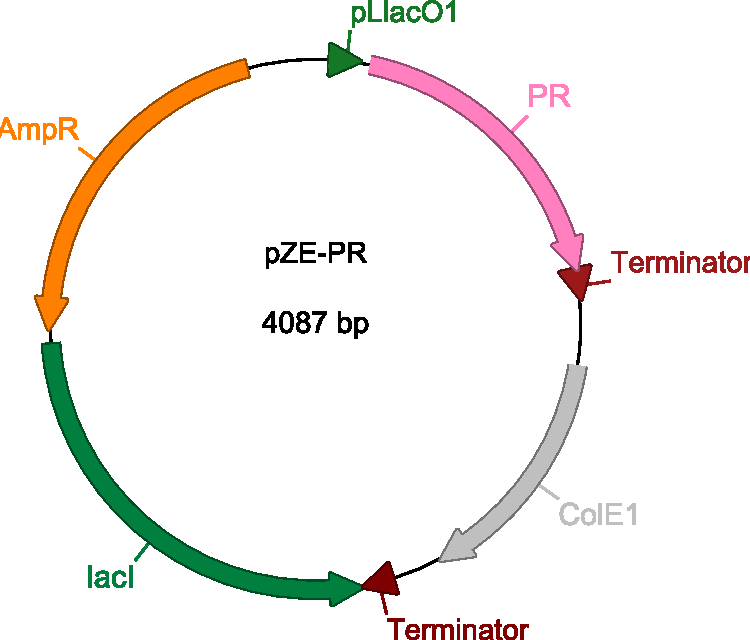
\includegraphics[width=3.5in]{Figs/A-1/1.pdf}
	%select pdftexify command to run jpg or pdf files
	\end{center}
	\caption[An illustration of pZE-PR plasmid]
	{
	An illustration of pZE-PR plasmid.
	}
	\label{fig:pze-pr}
\end{figure}
